\documentclass[tikz,border=5pt]{standalone}
\usetikzlibrary{intersections,spath3}
\begin{document}
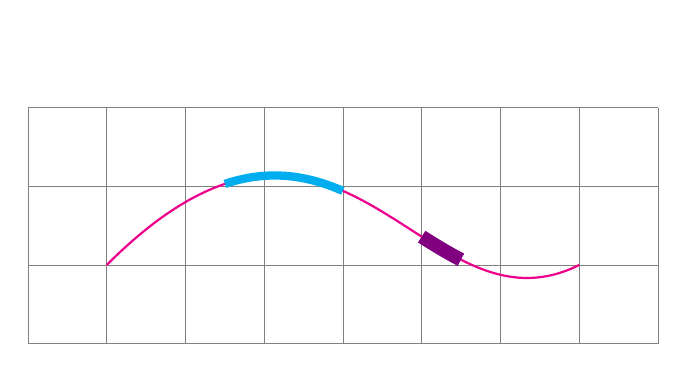
\begin{tikzpicture}
  \draw[help lines] (-1,-1) grid (7,2);
  \draw[thick,magenta,spath/save global=Curve]%<- define the curve
  (0,0) .. controls (3,3) and (4,-1) .. (6,0);
  \path[spath/save global=RectangleA] (1.5,-1) rectangle (3,3);
  \path[spath/save global=RectangleB] (4,-1) rectangle (4.5,3);
  \tikzset{%
    spath/.cd,
    clone={CurveForA}{Curve},%<- copy the curve
    split at intersections={CurveForA}{RectangleA},
    get components of={CurveForA}\curveComponentsA,
    clone={CurveForB}{Curve},%<- copy the curve
    split at intersections={CurveForB}{RectangleB},
    get components of={CurveForB}\curveComponentsB,
  }
  \draw[line width=3pt,cyan,spath/use=\getComponentOf{\curveComponentsA}{2}];
  \draw[line width=5pt,violet,spath/use=\getComponentOf{\curveComponentsB}{2}];
\end{tikzpicture}
\end{document}